\documentclass{beamer}

% Paquetes cargados
\usepackage{graphicx}
\usepackage[spanish]{babel}
\usepackage{ragged2e}
\usepackage{float} 
\usepackage{animate} 
\usepackage{media9}
\usepackage{caption}
\usepackage[T1]{fontenc}
\usepackage{lmodern}
\usepackage[utf8]{inputenc}
\usepackage{url}
\usepackage{lipsum}
\usepackage{bookmark}
\usepackage{hyperref}

% Paquetes para tablas y figuras
\usepackage{array}
\usepackage{booktabs}
\usepackage{tikz}
\usepackage{multicol}

% Paquetes matemáticos
\usepackage{amsmath}
\usepackage{mathtools}
\usepackage{amsfonts}
\usepackage{mathrsfs}
\usepackage{physics}
\usepackage{interval}

% Paquetes para colores
\usepackage{color}
\usepackage{colortbl}
\usepackage{transparent}

% Paquete para códigos
\usepackage{minted}
\usepackage{xcolor}

% --- CONFIGURACIÓN OPTIMIZADA PARA CÓDIGO CON MINTED ---
\setminted{
	fontsize=\tiny,           % Tamaño de fuente más controlado que \tiny
	bgcolor=orange!10,              % Color de fondo más sutil
	frame=lines,                    % Marco de líneas
	breaklines=true,                % Permite corte de líneas largas
	breakanywhere=true,             % Permite corte en cualquier lugar si es necesario
	linenos=true,                   % Números de línea
	numbersep=3pt,                  % Separación entre números y código
	%numberstyle=\tiny\color{gray!70}, % Estilo de números más sutil
	%captionpos=b,                   % Posición del caption
	style=friendly,                 % Estilo de coloreado
	tabsize=1,                      % Tamaño de tabulación
	xleftmargin=0pt,                % Margen izquierdo
	xrightmargin=0pt,               % Margen derecho
	resetmargins=true,              % Resetea márgenes
	autogobble=true,                % Elimina indentación automáticamente
	stripnl=true,                   % Elimina líneas vacías al inicio/final
	mathescape=false,               % Desactiva escape matemático para evitar conflictos
}

% Configuración específica para diferentes lenguajes
\newminted{r}{
	fontsize=\tiny,
	bgcolor=blue!5,
	frame=lines,
	breaklines=true,
	breakanywhere=true,
	linenos=true,
	numbersep=3pt,
	%numberstyle=\tiny\color{blue!50},
	style=friendly,
	tabsize=1,
	xleftmargin=0pt,
	xrightmargin=0pt,
	resetmargins=true,
	autogobble=true,
	stripnl=true,
}

% Entorno personalizado para código que se ajusta al ancho de la diapositiva
\newenvironment{codigoajustado}[1][r]{%
	\begin{adjustbox}{width=\textwidth,center}%
		\begin{minipage}{\textwidth}%
		}{%
		\end{minipage}%
	\end{adjustbox}%
}

% Paquete para ajustar contenido
\usepackage{adjustbox}

\captionsetup{justification=centering}

\hypersetup{
	pdfauthor={Nome Cognome},
	pdftitle={Titolo presentazione},
	pdfsubject={Argomento presentazione}
}

\title[EIG]{Especies de las Islas Galápagos}
\subtitle{Laboratorio de Modelos Lineales}
\institute{Universidad Católica del Maule}
\author[M.V]{Matías Valenzuela Nuche}
\year=2024
\month=10
\day=1

\def\relatore{José Zúñiga Núñez}
\def\relatoreLabel{Profesor}
\def\candidatoLabel{Autor}
\def\LogoDipartimento{otherResources/logo carrera.png}
\def\LogoFiligrana{otherResources/JAVI 4_Mesa de trabajo 1.png}
\def\LogoUniversita{otherResources/LOGO_IES.png}

%%%%%%%%%%%%%%%%%%%%%%%%%%%%%%%%%%%%%%%%%%%%%%%%%%%%%%%%%%%
%
% Copyright 2022 by Isac Pasianotto
%
% This file may be distributed and/or modified
%
% 1. under the LaTeX Project Public License and/or
% 2. under the GNU Public License.
%
%%%%%%%%%%%%%%%%%%%%%%%%%%%%%%%%%%%%%%%%%%%%%%%%%%%%%%%%%%%

%% 	Variabili di tipo "color": 

\definecolor{greenUnits100}{rgb}{0.0,0.5,0.0} 
\definecolor{greenUnits80}{rgb}{0.1,0.63,0.1}
\definecolor{greenUnits70}{rgb}{0.2,0.7,0.2}
\definecolor{greenUnits50}{rgb}{0.4,0.85,0.4}
\definecolor{greenUnits40}{rgb}{0.6,0.9,0.6}
\definecolor{greenUnits25}{rgb}{0.8,0.96,0.8}
\definecolor{greenUnits10}{rgb}{0.92,0.98,0.92}
\definecolor{grey}{rgb}{0.3686, 0.5255, 0.6235} 

%%	Palette di colori 

\setbeamercolor{palette primary}{bg=greenUnits100,fg=white}
\setbeamercolor{palette secondary}{bg=greenUnits80,fg=greenUnits25}
\setbeamercolor{palette tertiary}{bg=greenUnits50,fg=greenUnits100}
\setbeamercolor{palette quaternary}{bg=greenUnits40,fg=white}
\setbeamercolor{palette light primary}{bg=greenUnits25,fg=greenUnits100}
\setbeamercolor{palette titleframe}{bg=greenUnits10, fg=greenUnits80}


		%%%%%%%%%%%%%%%%%%%%%%%%%%%%%%%%%%
		%% Impostazioni generali slide  %%
		%%%%%%%%%%%%%%%%%%%%%%%%%%%%%%%%%%

%%	Setta l'immagine da mettere come sfondo, riducendone l'opacità
\usebackgroundtemplate{\tikz\node[opacity=0.1]{\includegraphics[height=\textheight]{\LogoFiligrana}};}

%%	Elenchi puntati, numerati, etc.

\setbeamercolor{structure}{fg=greenUnits80}
\setbeamertemplate{enumerate item}[circle]
\setbeamertemplate{itemize subitem}[ball]
% Valutare a secoda del contesto se sostituire con 
% \setbeamertemplate{items}[circle]
\setbeamercolor{alerted text}{fg=greenUnits50}

%% 	Colore delle scritte nella presentazione

\setbeamercolor{normal text}{fg=greenUnits100,bg=white}

%% 	Settaggio della linea in alto (headline)

\setbeamertemplate{headline}{
	\vskip1pt
	\leavevmode	
	\hbox{
		\begin{beamercolorbox}[wd=.99\paperwidth,ht=2.5ex,dp=1.125ex]{palette light primary}
			\insertsectionnavigationhorizontal{\paperwidth}{}{\hskip0pt plus1filll}
		\end{beamercolorbox}
	}
}

%%	Settaggio riga in basso (footline) 
 
\setbeamertemplate{footline}{
       \leavevmode
	   \hbox{
           \begin{beamercolorbox}[wd=.2\textwidth,ht=2.6ex,dp=1ex,center]{palette tertiary}
		    \usebeamerfont{author in head/foot}\insertshortauthor
    	\end{beamercolorbox}
	
    	\begin{beamercolorbox}[wd=.27\textwidth,ht=2.6ex,dp=1ex,center]{palette quaternary}
	   		\usebeamerfont{institute in head/foot}\insertshortinstitute
	   	\end{beamercolorbox}
	
    	\begin{beamercolorbox}[wd=.40\textwidth,ht=2.6ex,dp=1ex,center]{palette primary}
    		\usebeamerfont{title in head/foot}\insertshorttitle
    	\end{beamercolorbox}

    	\begin{beamercolorbox}[wd=.1\textwidth,ht=2.6ex,dp=1ex,center]{palette light primary}
	   		\insertframenumber{}/\inserttotalframenumber
	    \end{beamercolorbox}
    }
    \vskip2pt

}

%%	Settaggio tittoli delle slide  

\setbeamertemplate{frametitle}{
	\begin{beamercolorbox}[wd=\paperwidth,ht=2.75ex,dp=1ex,left]{palette titleframe}
		\qquad \textbf{\insertframetitle}
	\end{beamercolorbox}
}


		%%%%%%%%%%%%%%%%%%%%%%%%%%%%%%%
		%% Impostazioni Prima Slide  %%
		%%%%%%%%%%%%%%%%%%%%%%%%%%%%%%%
	
	
	
	
		
\def\setTitlestyleDissertation{
	
	\defbeamertemplate*{title page}{customized}[1][]{
		
		%  Commentare il seguente ambiente {center} e decommentare {flushright} quello successivo in caso
		%	si voglia usare solo il logo dell'UNI
		
		\begin{center}
			\begin{multicols}{2}
				\includegraphics[width=0.45\textwidth]{\LogoDipartimento}
			\columnbreak
				\includegraphics[scale=0.145]{\LogoUniversita}		
			\end{multicols}
		\end{center}
	
		%	\begin{flushright}
		%		\includegraphics[width=0.45\textwidth]{\LogoUniversita}	
		%	\end{flushright}
	
		\smallskip
		
		\begin{center}		
			\usebeamerfont{title}\textbf{\inserttitle}\par
			\usebeamerfont{subtitle}\usebeamercolor[fg]{subtitle}\insertsubtitle\par
			\medskip		
			
			%% Il seguente layout dentro l'ambiente multicols serve per le tesi.
			
			\begin{multicols}{2}
				\begin{tabular}{c}
					\usebeamerfont{normal text}{\relatoreLabel} \\
					\usebeamerfont{author}{\relatore}
					
						% Decommentare in caso siano presenti dei correlatori
					%\\
					%\usebeamerfont{normal text}{\correlatoreLabel} \\
					%\usebeamerfont{author}{\correlatore}
						
				\end{tabular}					
				\columnbreak
				\begin{tabular}{c}
					\candidatoLabel \\
					\usebeamerfont{author}{\insertauthor}
				\end{tabular}
			\end{multicols}
		
			\par
			
			\bigskip  	% --> nel caso di relatore e basta
			%\smallskip 	% --> nel caso di relatore + correlatore
			
			\insertinstitute\par
			
			\bigskip	% --> nel caso di relatore e basta
			%\smallskip	% --> nel caso di relatore + correlatore
			
			\usebeamerfont{date}\insertdate\par
			
			\bigskip	% --> nel caso di relatore e basta
			%\smallskip	% --> nel caso di relatore + correlatore
		\end{center}
	}
}


\begin{document}
	
	\begin{frame}
		\setTitlestyleDissertation
		\maketitle
	\end{frame}
	
	\begin{frame}[fragile]
		\frametitle{Contenidos}
		\justifying
		\tableofcontents
	\end{frame}
	
	\section{Introducción}
	\begin{frame}[fragile]
		\frametitle{Introducción}
		\justifying
		
		\begin{itemize}
			\item Las islas Galápagos constituyen un archipiélago del océano Pacífico, ubicado a 972 km de la costa de Ecuador.
			\item Estas islas son conocidas por sus numerosas especies endémicas y por los estudios de Charles Darwin sobre la teoría de la evolución por selección natural.
			\item En estas islas se han registrado 55 de las más grandes erupciones volcánicas de los últimos tiempos.
		\end{itemize}
		
		\vspace{0.2cm}
		
		\begin{figure}[h] 
			\centering 
			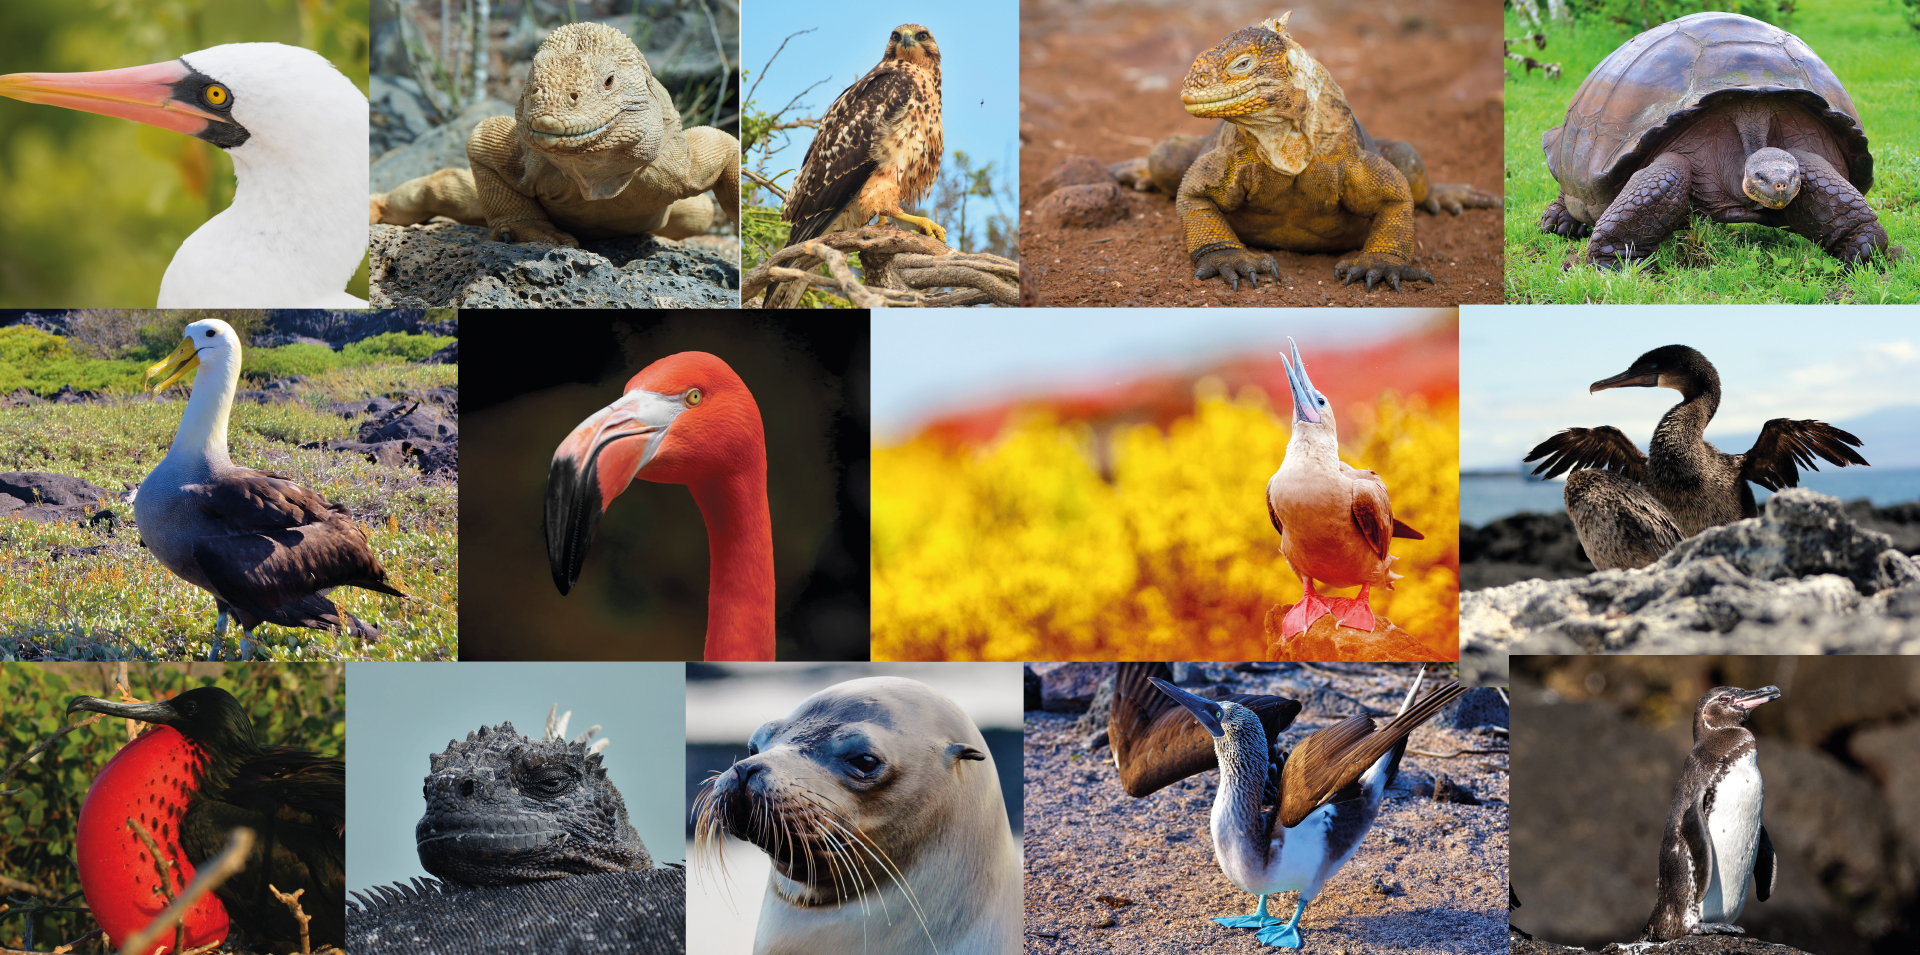
\includegraphics[width=0.5\textwidth]{big-15-galapagos-iconic-species.jpg}
			\caption{Especies icónicas de las islas Galápagos.}  
			\label{fig:Especies}  
		\end{figure}    
	\end{frame}
	
	\section{Descripción}
	\begin{frame}[fragile]
		\frametitle{Descripción}
		\justifying
		
		Se busca encontrar patrones ecológicos que sean capaces de predecir la diversidad de especies de una isla del archipiélago cualquiera, basándonos en sus relaciones de frecuencias con otros factores ecológicos registrables.
		
		\vspace{0.2cm}
		
		\noindent
		\begin{minipage}[t]{0.6\textwidth}
			\begin{itemize}
				\item Ernst Haeckel (1834-1919), como acuñador del término <<\textbf{ecología}>>, lo define como \textit{las interacciones entre los organismos y su medio ambiente}.
				\item Esto refleja que las condiciones físicas del nicho ecológico son claves para el entendimiento de un ecosistema.
			\end{itemize}
		\end{minipage}
		\hfill
		\begin{minipage}[t]{0.3\textwidth}
			\begin{figure}[h]
				\centering
				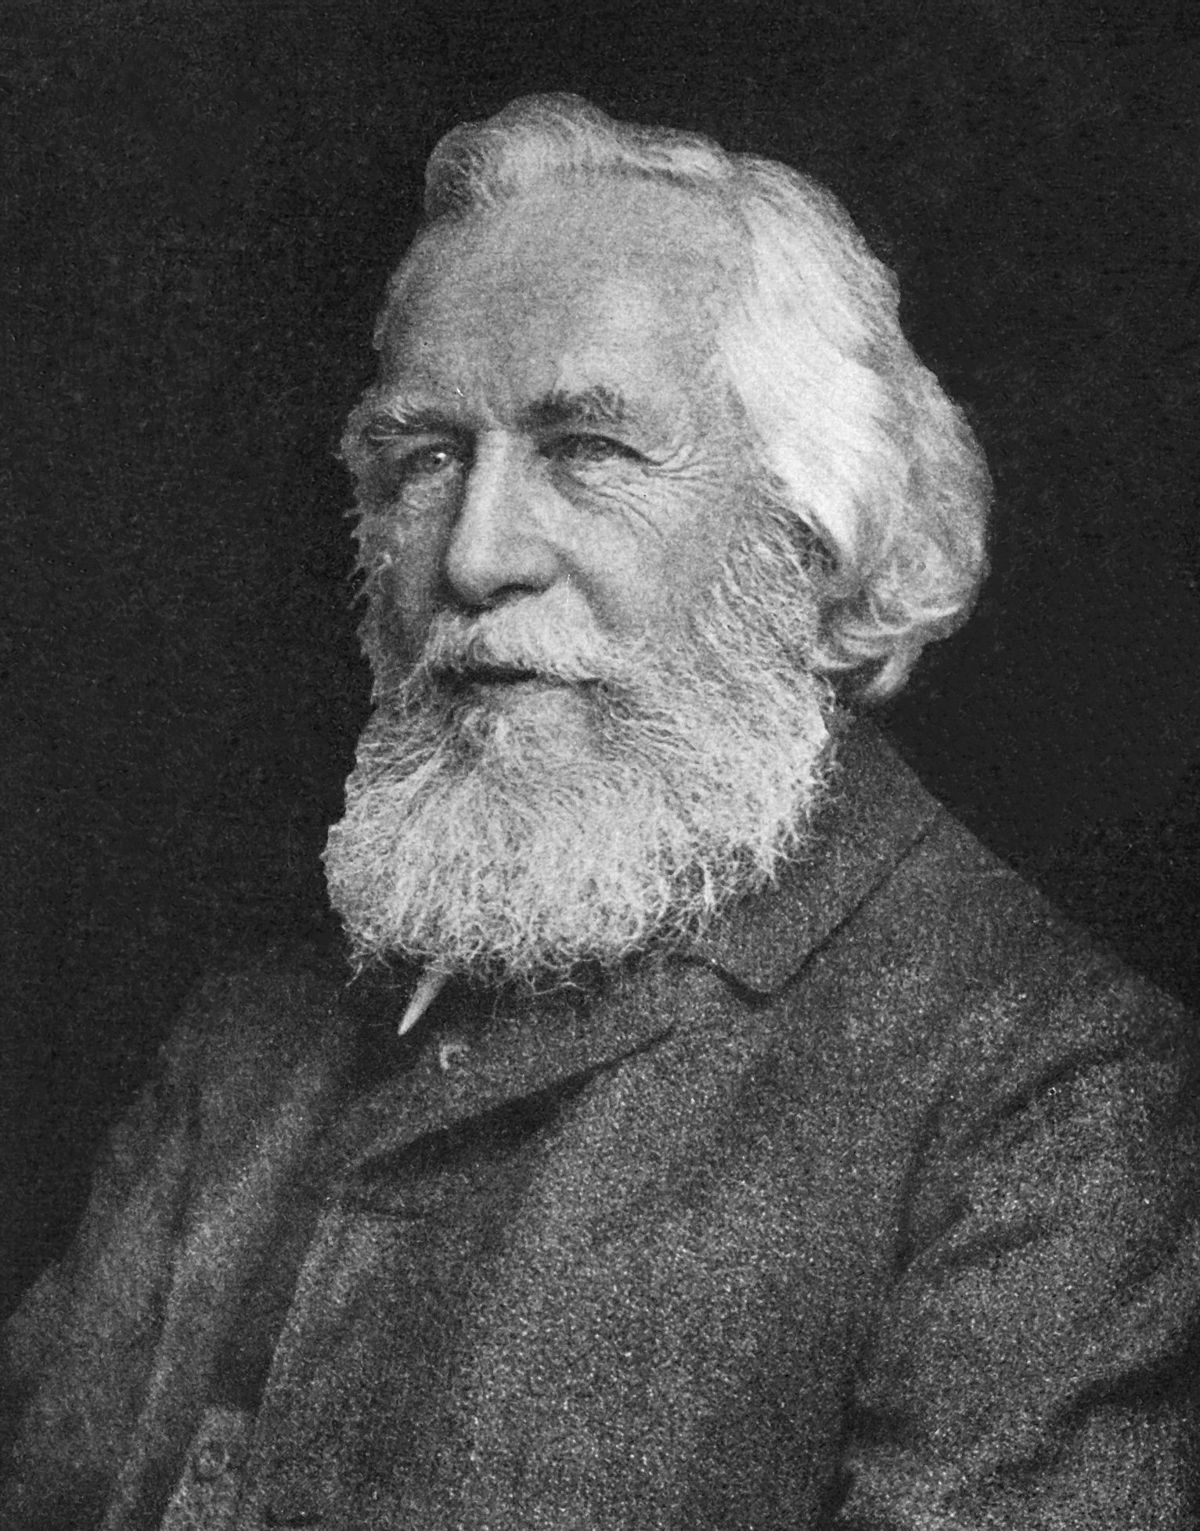
\includegraphics[width=\textwidth]{1200px-Ernst_Haeckel_5.jpg}
				\caption{Ernst Haeckel}
				\label{fig:Ernst_Haeckel}
			\end{figure}
		\end{minipage}
	\end{frame}
	
	\begin{frame}[fragile]
		\frametitle{Descripción}
		\justifying
		
		Se dispone de información sobre 25 islas del archipiélago, recolectada en la actualidad, y contiene las siguientes variables:
		
		\vspace{0.2cm}
		
		\begin{itemize}
			\item \textbf{isla}: nombre de la isla. [Nominal] [Id.]
			\item \textbf{numero}: número de especies presentes en la isla. [Razón] [Discreta]
			\item \textbf{area}: área de la isla ($km^2$). [Razón] [Continua]
			\item \textbf{elevacion}: altitud de la isla sobre el nivel del mar ($m$). [Razón] [Continua]
			\item \textbf{cercana}: distancia a la isla más próxima ($km$). [Razón] [Continua]
		\end{itemize}
	\end{frame}
	
	\begin{frame}[fragile]
		\frametitle{Descripción}
		\justifying
		
		\begin{figure}[h]
			\centering
			\begin{minipage}[b]{0.34\textwidth}
				\centering
				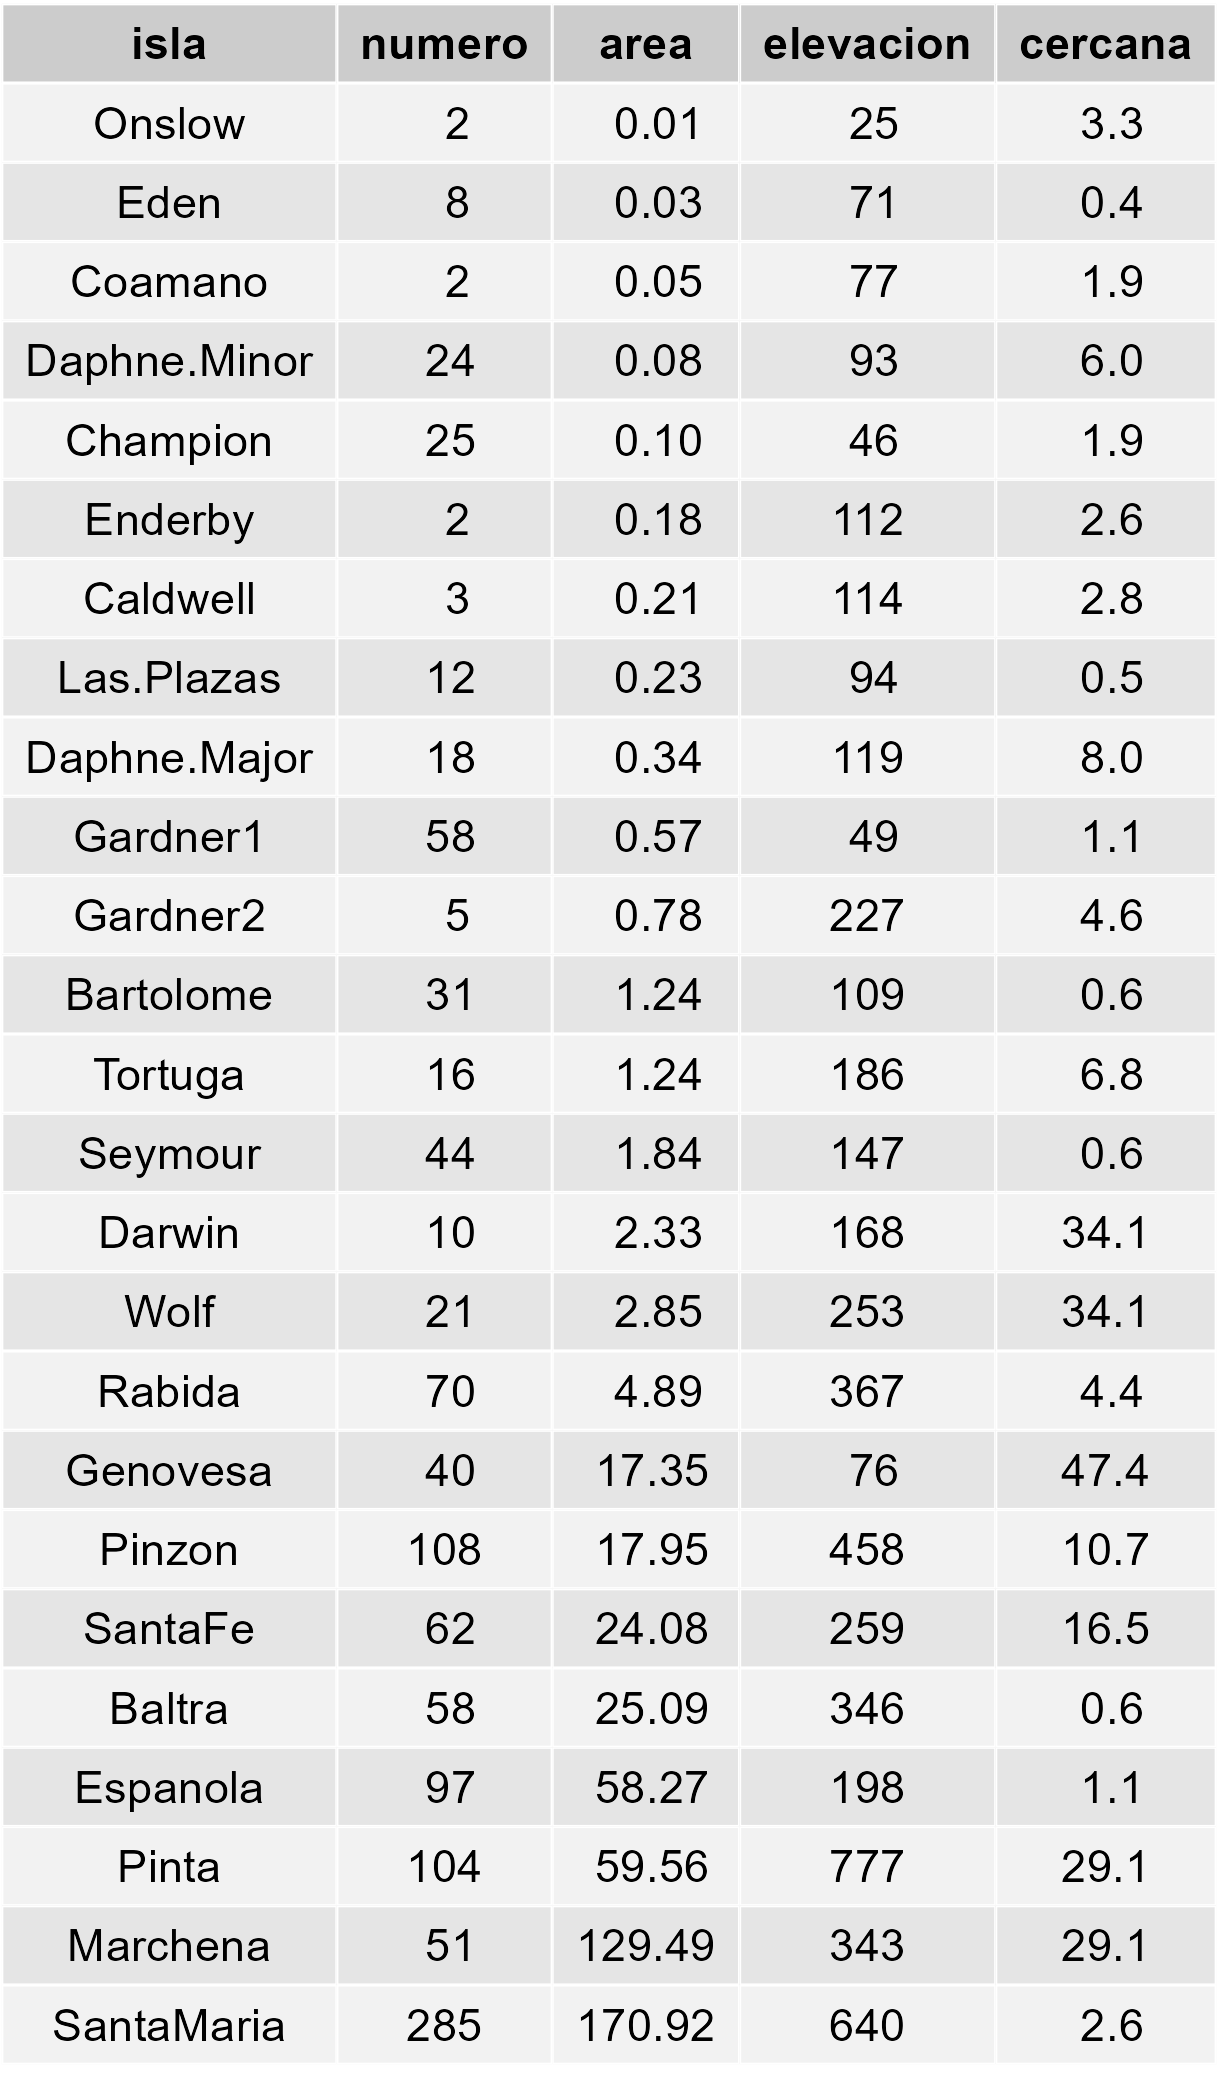
\includegraphics[width=\textwidth]{tabla_base_datos.png}
				\caption{Base de Datos disponibles.}
				\label{fig:mapa1}
			\end{minipage}
			\hfill
			\begin{minipage}[b]{0.64\textwidth}
				\centering
				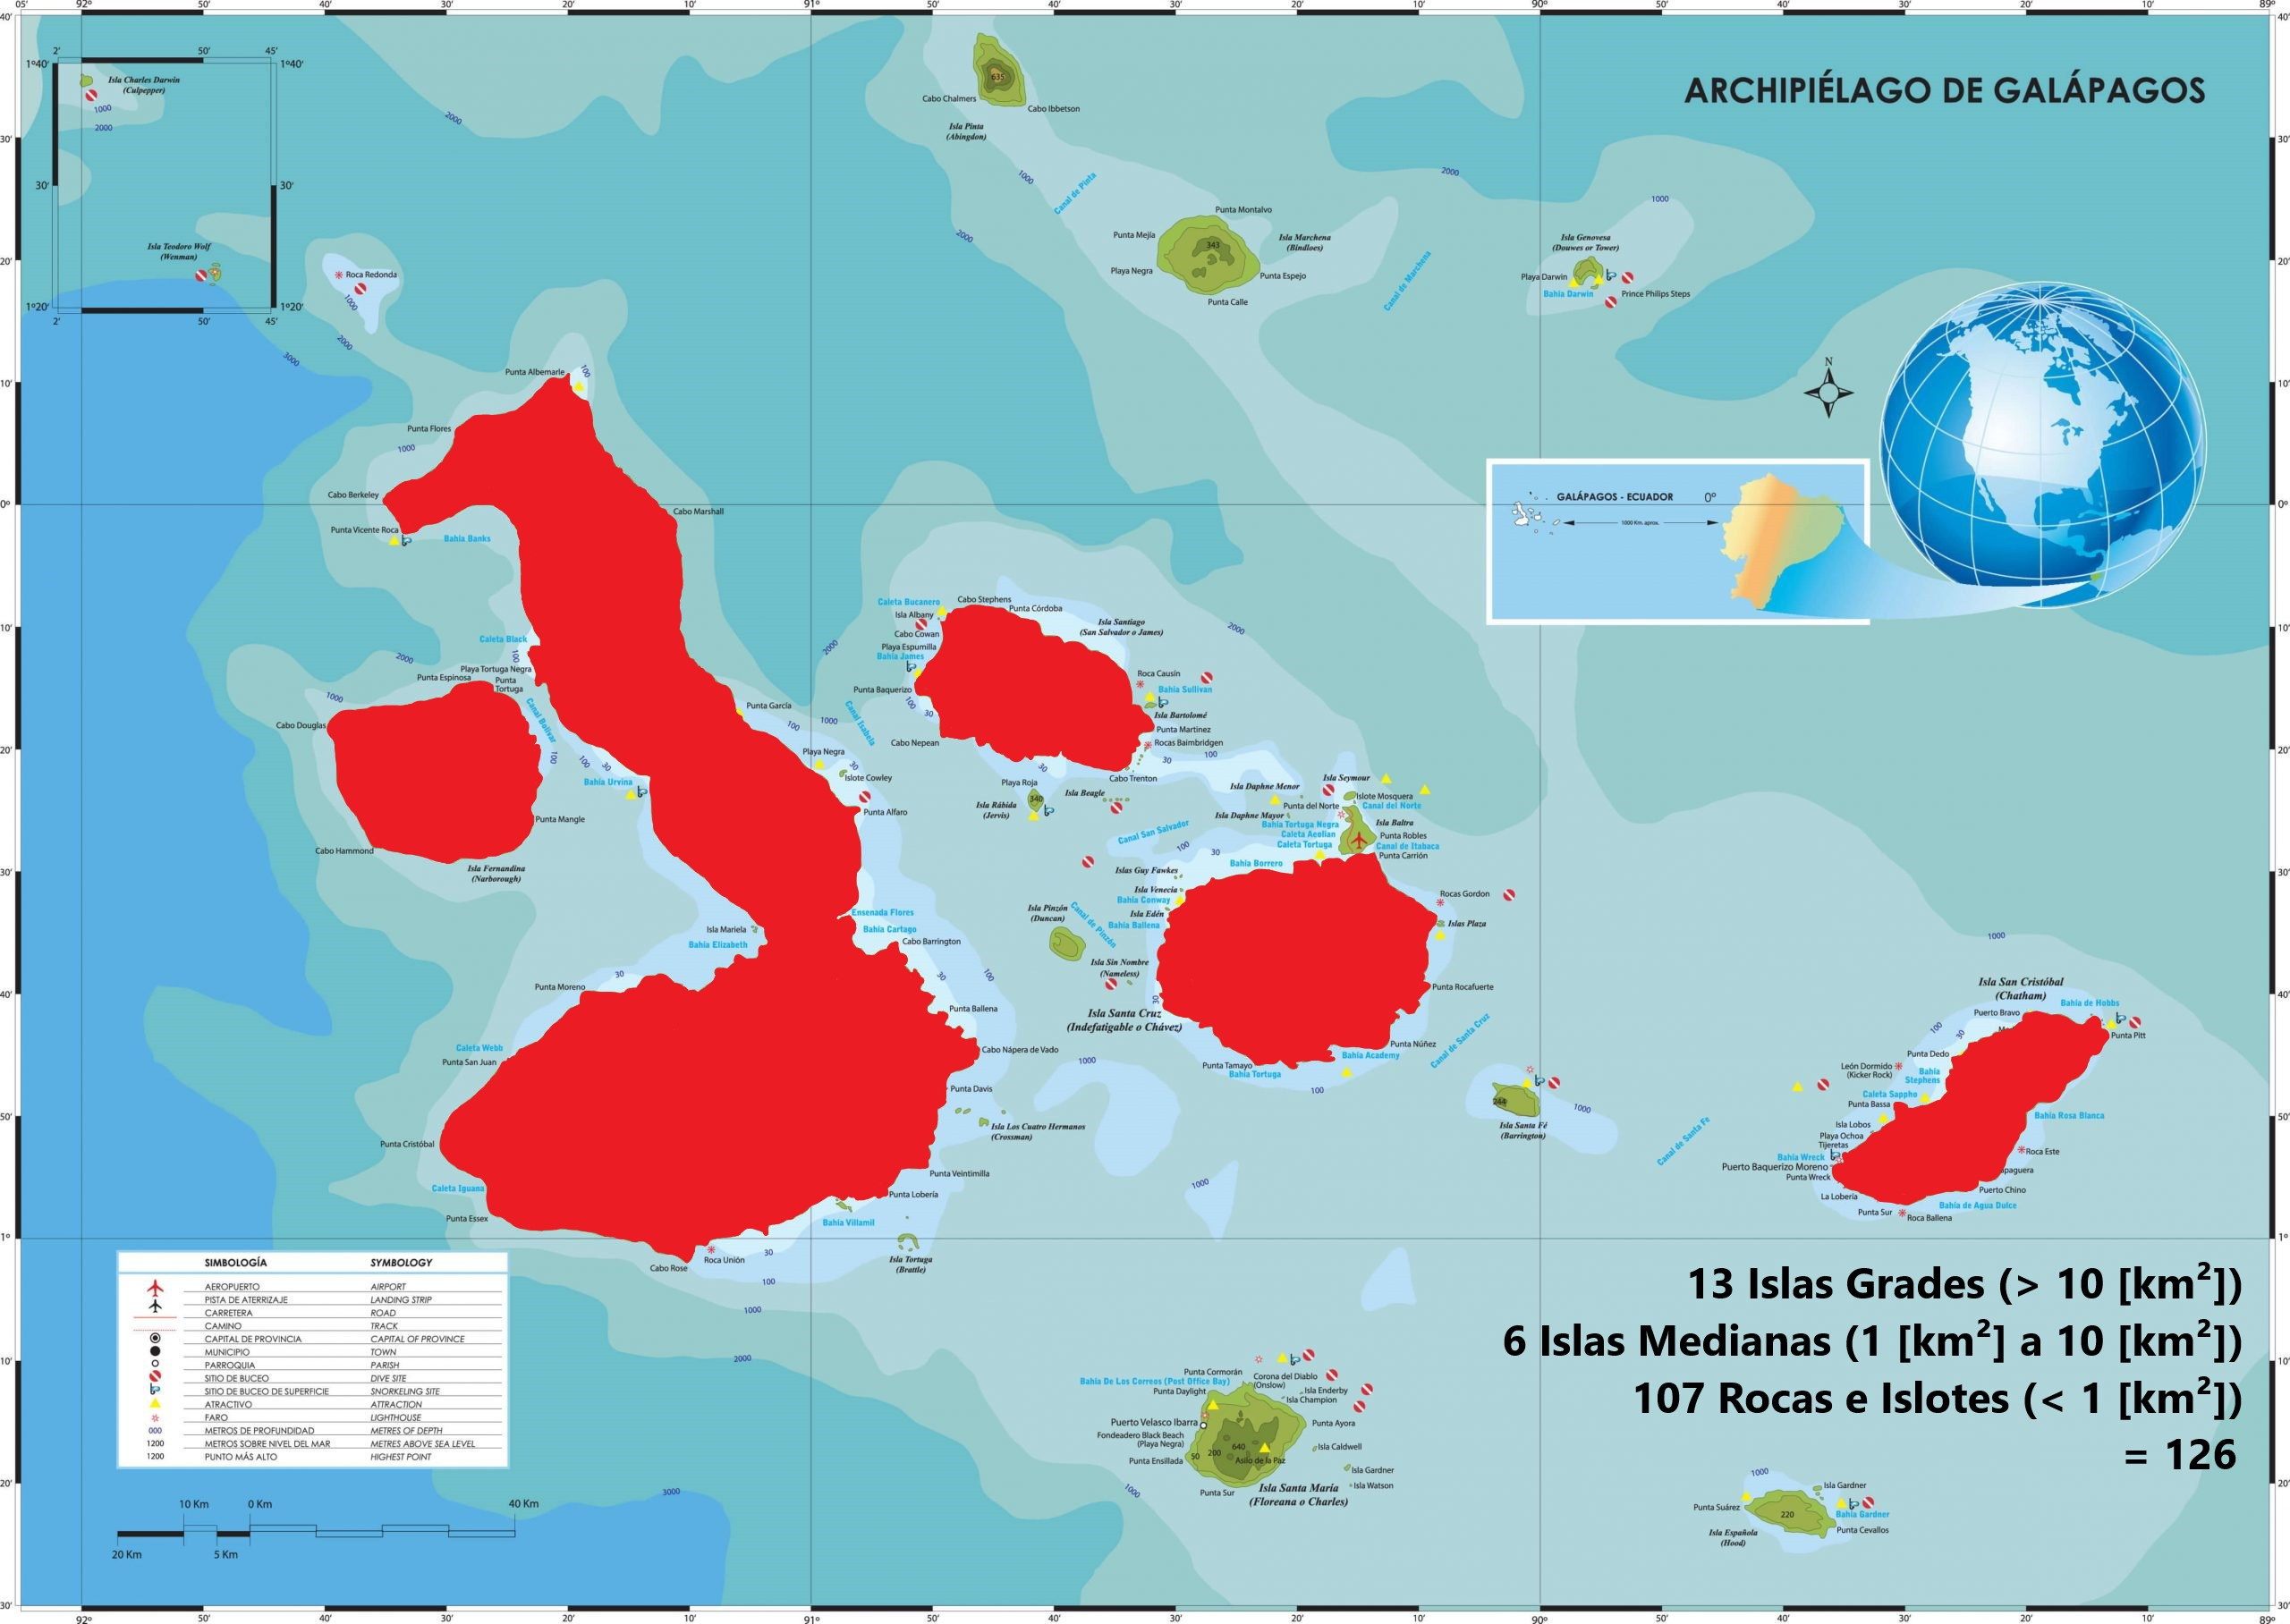
\includegraphics[width=\textwidth]{mapa-galapagos-scaled.jpeg}
				\caption{Mapa de Galápagos. En rojo, islas no consideradas.}
				\label{fig:mapa2}
			\end{minipage}
		\end{figure}
	\end{frame}
	
	\section{Análisis preliminar}
	\begin{frame}[fragile]
		\frametitle{Análisis preliminar}
		\justifying
		
		\begin{codigoajustado}
			\begin{rcode}
				pairs(df2, pch = 19, col = 6, 
				main = "Pareado de variables ecologicas", 
				gap = 0.2, row1attop = FALSE, 
				labels = colnames(df2), 
				cex.labels = 1.8, font.labels = 1)
			\end{rcode}
		\end{codigoajustado}
		
		\vspace{0.3cm}
		
		\begin{figure}[h]
			\centering
			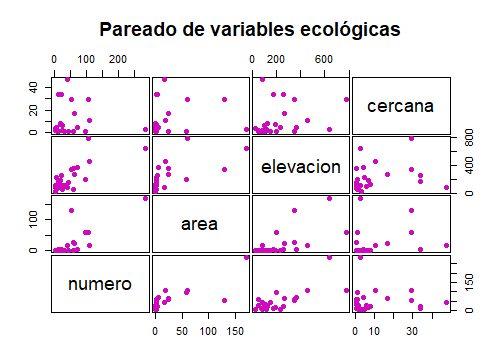
\includegraphics[width=0.75\textwidth]{Rplot03.png}
			\label{fig:Pair}
		\end{figure}
	\end{frame}
	
	\begin{frame}[fragile]
		\frametitle{Análisis preliminar}
		\justifying
		
		\begin{codigoajustado}
			\begin{rcode}
				library(ggplot2)
				library(tidyr)
				library(dplyr)
				cor_matrix <- cor(df2, method = "pearson")
				cor_long <- as.data.frame(as.table(cor_matrix))
				ggplot(data = cor_long, aes(Var1, Var2, fill = Freq)) + 
				geom_tile(color = "white") + 
				scale_fill_gradient2(low = "blue", high = "red", 
				mid = "purple", midpoint = 0, 
				limit = c(-1, 1), name = "Correlacion") + 
				theme_minimal() + 
				labs(title = "Heatmap de Correlacion", x = "", y = "") + 
				geom_text(aes(label = round(Freq, 2)), 
				color = "white", size = 5)
			\end{rcode}
		\end{codigoajustado}
		
		\vspace{0.2cm}
		
		\begin{figure}[h]
			\centering
			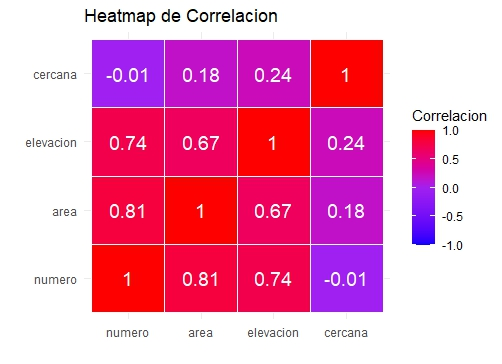
\includegraphics[width=0.55\textwidth]{Rplot04.jpeg}
			\label{fig:Heat}
		\end{figure}
	\end{frame}
	
	\section{Modelado}
	\begin{frame}[fragile]
		\frametitle{Modelado}
		\justifying
		
		\textbf{Regresión lineal multiple}
		
		\vspace{0.2cm}
		
		\begin{equation*}
			Y = X\beta + \epsilon \text{,   } \epsilon \sim N(0, \sigma^2I)
		\end{equation*}
		
		Donde:
		
		\begin{itemize}
			\item $Y$: vector de valores de la variable dependiente de orden $n \times 1$.
			\item $X$: matriz "de diseño" de orden $n \times p$ correspondiente a los valores de las variables independientes.
			\item $\beta$: vector de orden $p \times 1$ de parametros llamados \textit{coeficientes de regresión}.
			\item $\epsilon$: vector de errores aleatorios de orden $n \times 1$.
			\item $\sigma^2$: varianza de la distribución Normal.
			\item $I$: matriz identidad de orden $n \times n$.
		\end{itemize}
	\end{frame}
	
	\begin{frame}[fragile]
		\frametitle{Modelado}
		\justifying
		
		\begin{columns}
			\begin{column}{0.45\textwidth}
				\textbf{Ajuste del modelo}
				
				\vspace{0.2cm}
				
				\begin{rcode}
					X <- cbind(df$area, df$elevacion, df$cercana)
					dim(X) # 25 3
					n <- dim(X)[1]
					p <- dim(X)[2]
					v <- rep(1,n)
					X <- cbind(v, X)
					dim(X) # 25 4
					X[2,3] # 71
					df[2,1] # "Eden"
					Y <- df$numero
					B <- solve(t(X) %*% X) %*% t(X) %*% Y
					val_pred <- X %*% B
					cor(Y,val_pred) # 0.87
					
					plot(Y, val_pred, 
					xlab = "Valores Observados", 
					ylab = "Valores Predichos", 
					col = "blue", pch = 16)
					abline(0, 1, col = "red")
				\end{rcode}
			\end{column}
			
			\begin{column}{0.55\textwidth}
				\centering
				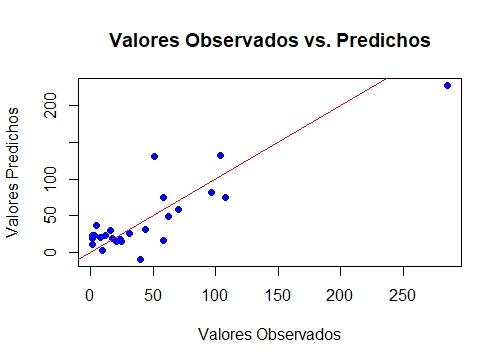
\includegraphics[width=\textwidth]{Rplot05.jpeg}
			\end{column}
		\end{columns}
		
		\vspace{0.2cm}
		
		\begin{equation*}
			\hat{\beta}_0 = 11.09,\text{ } \hat{\beta}_1 = 0.79,\text{ } \hat{\beta}_2 = 0.13,\text{ } \hat{\beta}_3 = -0.91
		\end{equation*}
	\end{frame}
	
	\begin{frame}[fragile]
		\frametitle{Modelado}
		\justifying
		
		\begin{columns}
			\begin{column}{0.5\textwidth}
				\textbf{Cálculo de incertidumbre}
				
				\vspace{0.2cm}
				
				\begin{rcode}
					e <- Y - B %*% X
					H <- X %*% solve(t(X) %*% X) %*% t(X)
					I <- diag(1,n)
					SCE <- t(Y) %*% (I - H) %*% Y
					sig <- SCE/(n-p)
					sig_scal <- as.numeric(sig)
					sigb <- solve(t(X) %*% X) * sig_scal
					sqrt(sigb[2,2]) # 0.192
					rownames(sigb) <- c("intercepto", "area", 
					"elevacion", "cercania")
					colnames(sigb) <- c("intercepto", "area", 
					"elevacion", "cercania")
					sigb_long <- as.data.frame(as.table(sigb))
					ggplot(data = sigb_long, 
					aes(Var1, Var2, fill = Freq)) + 
					geom_tile(color = "white") + 
					scale_fill_gradient2(low = "blue", high = "red", 
					mid = "purple", midpoint = 0, 
					limit = range(sigb), 
					name = "Covarianza") + 
					theme_minimal() + 
					labs(title = "Matriz de Covarianzas de Coeficientes", 
					x = "", y = "") + 
					geom_text(aes(label = round(Freq, 3)), 
					color = "white", size = 5)
				\end{rcode}
			\end{column}
			
			\begin{column}{0.5\textwidth}
				\centering
				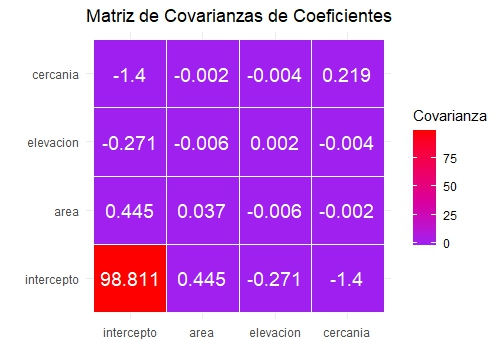
\includegraphics[width=\textwidth]{Rplot06.jpeg}
			\end{column}
		\end{columns}
	\end{frame}
	
	\section{Conclusión}
	\begin{frame}[fragile]
		\frametitle{Conclusión}
		\justifying
		\centering
		\Huge
		\textbf{Conclusión}
	\end{frame}
	
	\section{Bibliografía}
	\begin{frame}[fragile]
		\frametitle{Bibliografía}
		\justifying
		\begin{itemize}
			\item Aprenda estadísticas fácilmente. (2023, 13 de junio). \textit{Una guía completa sobre los niveles de medición en el análisis de datos}. \url{https://es.statisticseasily.com/niveles-de-medida/}
			\item Ecuador Ec. (s.f.). ¿Cuántas islas hay en Galápagos? ¿Cuáles son los nombres?. \url{https://ecuadorec.com/cuantas-islas-hay-en-galapagos-cual-son-los-nombres/}
			\item Ecuador Galápagos Info. (s.f.). \textit{Mapa de Galápagos}. \url{https://ecuadorgalapagosinfo.com/islas-galapagos/mapa/}
			\item Rodríguez Martínez, J. (2013). \textit{Ecología} (3a ed.). Ediciones Pirámide.
			\item Ximénez, M. C., \& San Martín, R. (2013). \textit{Fundamentos de las técnicas multivariantes}. Universidad Nacional de Educación a Distancia. Edición digital, octubre de 2013.
		\end{itemize}
	\end{frame}
	
\end{document}